\section{Static-Network Analysis}

\subsection{Statistics}

\subsubsection{Small World}
At the book's end, the largest component has 224 nodes and the diameter is 5.
Since $ln(224) = 5.41$, we see that this network does indeed display the small world property, similar to real-world social networks.

\subsubsection{Degree Distribution}

\begin{figure*}[t]
    \centering
    \begin{subfigure}{0.4\textwidth}
        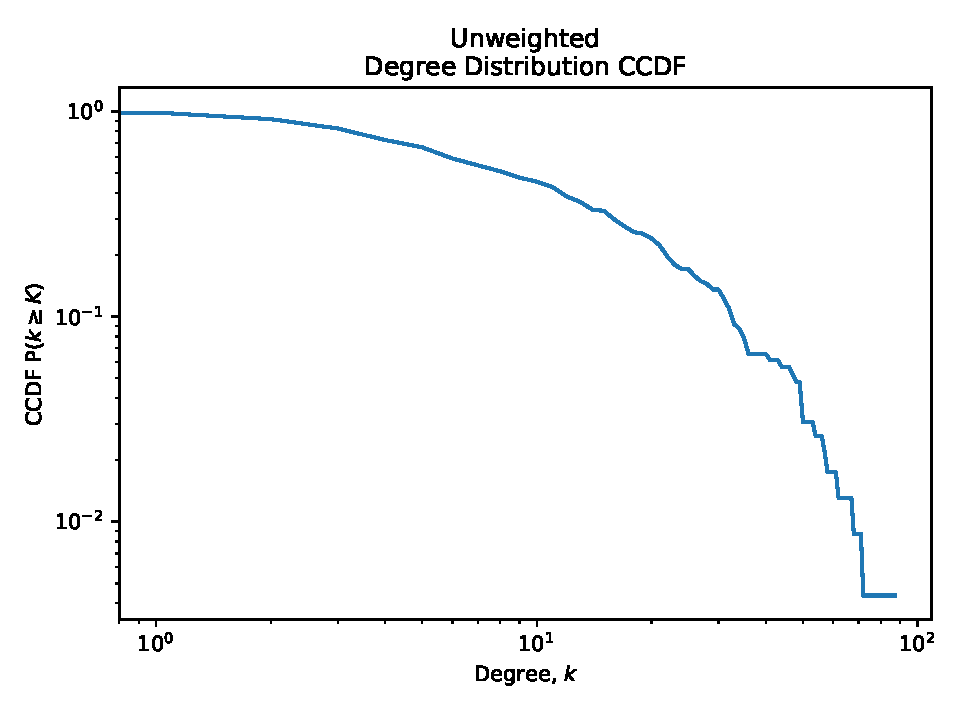
\includegraphics[width=1.\textwidth]{images/unweighted_degree_distr_ccdf.pdf}
        \caption{Unweighted degree distribution.}
    \end{subfigure}
    ~
    \begin{subfigure}{0.4\textwidth}
        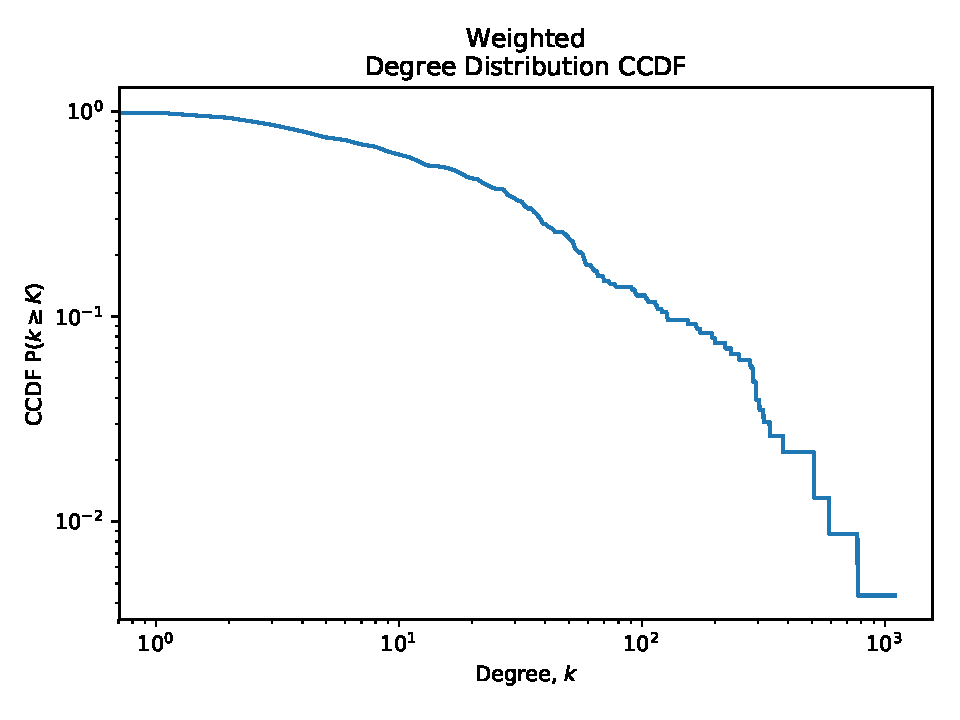
\includegraphics[width=1.\textwidth]{images/weighted_degree_distr_ccdf.pdf}
        \caption{Weighted degree distribution.}
    \end{subfigure}
    \caption{Degree distributions on a log-log scale. Though we do observe a heavy tail, we do not see a power law.}
    \label{fig:degree_distr}
\end{figure*}

The degree distributions for the weighted and unweighted networks are shown as a CCDF in Figure \ref{fig:degree_distr}. We see a heavy tail like we might expect from many real-world networks, but neither appear to show a power law in the tail. 

In the unweighted network in particular we see a distribution that clearly has more high-degree nodes than expected under a Poisson random graph, yet the tail drops of much faster than expected in a scale-free network.
The weighted degree distribution shows a heavier tail than the unweighted one, suggesting the distribution of character mentions within the book is much more uneven than the unweighted graph of character interactions. The weighted network is closer to a power law, though we still hesitate to call it scale-free.

%$P(k) \sim k^{-\tau}$, or power law with a cutoff, $P(k) \sim k^{-\tau}10^{-k/c}$

We can only speculate on the attachment mechanism behind the degree distribution, leaving testing such hypothesis to future work. Since the degree distribution does not follow a power law, vertex copying and preferential attachment do not make sense. 
Perhaps main characters are introduced in the beginning, and the book does not contain many minor throw-away characters.

The average degree is 13.31 and the average weighted degree is 55.95

\subsubsection{Assortativity}
We see an unweighted degree assortative mixing coefficient of -0.0945.
Degree assortative networks typically reflect core-periphery structures, where a dense core of highly-connected nodes is surrounded by successively less-dense periphery nodes. Degree disassortative networks, on the other hand, are more stars with high-degree nodes connected to low-degree. 
According to Newman in {\em Networks}, social networks are unusual in that they typically have a positive degree assortativity \cite{NewmanBook}. 
Therefore it is strange for us to see disassortative mixing by degree in \infinitejest, possibly indicating more of a star-like structure or fewer community structures than real-world social networks.

\subsection{Modularity}

- talk about NMI
- talk about modularity

\subsubsection{Clustering}
Using the transitivity definition of clustering coefficient, we can examine the fraction of closed triads.
$$ C = \frac{\text{(number of triangles)} \cdot 3}{\text{number of connected triples}} $$

This metric disregards the edge weights, looking only at connections between characters. We find $C = 0.3930$, reflecting the relatively dense connections -- perhaps within communities such as the Tennis Academy or Halfway House -- as opposed to a tree-like structure rooted at the highest-degree (main) characters.

We can compare the clustering coefficient against the configuration model to determine if this effect is due to the degree sequence alone or perhaps reflects a conscious author choice. We find configuration model we get an average local clustering coefficient of 0$.1728$, vs $0.3930$ in the book. 

TODO: how does this compare to real social networks?

\subsection{Gender}

